\documentclass[a4paper]{article}
\usepackage[T1]{fontenc}
\usepackage[utf8]{inputenc}
\usepackage[english]{babel}
\usepackage{amssymb}
\usepackage{hyperref}
\usepackage{mathtools}
\usepackage{amsthm}
\usepackage{varioref}

\mathtoolsset{showonlyrefs}  
\hypersetup{
    colorlinks=true,
    linkcolor=black,
    filecolor=black,      
    urlcolor=black,
}

\newcommand{\pluseq}{\mathrel{{+}{=}}}

\newtheorem{theorem}{Theorem}
\newtheorem{corollary}{Corollary1}
\newtheorem{lemma}{Lemma}
\newtheorem*{remark}{Remark}
\newtheorem{definition}{Definition}

\setcounter{secnumdepth}{3}
\setcounter{tocdepth}{3}

\title{Information retrieval}
\author{Francesco Tomaselli}
\makeindex
\begin{document}
\maketitle
% \newpage
\tableofcontents
\setlength{\parindent}{0pt}
\setlength{\parskip}{0.8em}
\newpage

\section{Vector space model}
\label{vect-vect-model}

\paragraph{Text transformation}
The first step to process queries on text is to transform 
it into a model that can be computed by a machine.

Such a model should be suitable for any kind of text, should be able 
to capture the semantic of words and then should support the notion of
\emph{text similarity}.

The main idea of a vector space model is to map documents in a vector, 
so they appear as points in a certain space.

For instance, we can collect some words and index them, then build a vector 
for each document $$d_k = [x_0, \dots, x_n]$$
where the value $x_i$ stores the occurrences of the word indexed with $i$ 
in that document.

\paragraph{Similarity} 
This model somehow implements the notion of text similarity, represented 
by some sort of distance function between two documents in space, perhaps 
the \emph{Euclidean distance} or the difference between the angle of the two 
vectors.
There are a lot of distance measures, and they vary in applications.
Some of them assume normalization in the document vectors.


\paragraph{Document-Term matrix}
If we arrange document vectors in a vector we obtain the 
\emph{document-term matrix}, or the \emph{term-document matrix} if 
we take the opposite.
The number of dimensions in the space is equal to the 
number of words in the vocabulary. \\
That can be a problem without some sort of lemmatisation and stemming, 
as sparsity and dimension of the matrix increases.

\paragraph{Vector length problem}
By considering the length of the vector in a similarity measure, 
we are introducing some problems, let's just consider a text and its 
abstract, the Euclidean distance would be huge, as most of the words do not 
appear that often. \\
To solve the problem we can consider the \emph{Cosine similarity} or 
normalize vector lengths.

The main phases in the generation of a vector space models are:
tokenization, normalization, weight, and indexing.

\subsection{Tokenization}
The goal is to split the text in words, for instance we could split the
document at the spaces.

In practice this can be obtained with \emph{Regex}, \emph{Corpus} based and \emph{Machine Learning} based
methods.
\subsection{Normalization}
\label{normalization}
The idea is to normalize each token, that could mean writing verbs in the normal 
form, or plurals at the singular.

\paragraph{Stemming}
One form of normalization is stemming, that simply truncate words 
to obtain singular or infinite forms.
The problems here could be creation of meaningless words and also 
close words in meaning could be completely different. An example
is the \emph{Porter} stemming algorithm.

\paragraph{Lemmatisation}
Another way to normalize is to lemmatise, 
It's similar to stemming, but the words are replaced with the dictionary 
root, this also has a problem, indeed sometime mapping of same words to 
different lemmas can happen. A way to lemmatise is to use a 
\emph{Dictionary based} lemmatisation, or something more complicated 
such as \emph{Wordnet}.

\paragraph{Wordnet}
Wordnet is a large lexical database, verbs, nouns, adjectives and adverbs are
grouped into cognitive synonyms, called synsets, each expressing
a different concept.
Synsets are connected to each other by conceptual relations and they are also 
connected to a lemma.

\subsection{Term Weighting}
Weighting the words is a crucial point in text processing, 
an easy way could be counting the frequency of the terms in the document.

\paragraph{Term frequency}
An example of weighing is the term frequency, 
which counts the frequency of a term given a document:
\begin{itemize}
    \item \emph{Boolean}: so a 0 or 1 if the word is present or not
    \item \emph{Natural}: $\mathit{tf}_{t,d} = $  count of a specific word
    \item \emph{Log}: $1 + \log(\mathit{tf}_{t,d})$
    \item \emph{Augmented}: $0.5 + \frac{0.5\mathit{tf}_{t,d}}{\max_{t^\prime} \mathit{tf}_{t^\prime,d}}$
    \item \emph{Log average}:  $0.5 + \frac{0.5 \log(\mathit{tf}_{t,d})}{1 + \log(\mathit{avg}_{t^\prime} \mathit{tf}_{t^\prime,d})}$
    \item \emph{Max tf norm}: $k + (1-k)\frac{\mathit{tf}_{t,d}}{\mathit{tf}_{\max}(d)}$
\end{itemize}

\paragraph{Stop words problem}
A problem in this model is the excessive presence of stop words and punctuations.
To compensate, we can remove them in the normalization phase. \\
But sometimes the stop words can be important, for instance with phrasal verbs.
A solution can be to count the number of documents that contains that given word.

\paragraph{Inverse document frequency}
The idea is to count the number of documents that contains a 
given words, and to prefer less frequent words: $$\mathit{idf} = \log\frac{N}{\mathit{df}_t}$$
There are many variants: 
\begin{itemize}
    \item \emph{Smooth}: $\log(\frac{N}{1 + \mathit{df}_t}) + 1$
    \item \emph{Max}: $\log(\frac{\max_{t^\prime \in d} \mathit{df}_t}{1 + \mathit{df}_t}) + 1$
    \item \emph{Probabilistic}: $\log \frac{N - \mathit{df}_t}{\mathit{df}_t}$
\end{itemize}

\paragraph{TfIdf}
By multyplying term frequency and inverse term frequency we obtain this metric.
$$TfIdf(t, d) = \mathit{tf}_{t,d} \cdot \mathit{idf}_t$$
Regarding the value of terms:
\begin{itemize}
    \item the terms with a high \emph{TfIdf} usually appears in a small number of documents
    \item the metric is low when a term appears a few times in a document or when it appears in 
    many documents
\end{itemize}
\section{Evaluation on retrieval systems}

The goal of evaluation is to assess the quality of the results 
obtained by an IR system.
There's the need of knowing a \emph{ground truth}, so an annotated corpus 
where for each task we know what documents are relevant. The annotations
could be created manually or derived from the data, if it contains 
annotations.

\subsection{The notion of quality}
Given a corpus $C$ and a query $q$, the task is to find a set of 
documents $A_{q,C}$ that match $q$, but after retrieving such documents, 
there's the need to estimate the quality of results.

\paragraph{Precision}
To formalise the quality of the retrieved documents $A_{q,C}$ we could 
count how many of these documents are relevant to $q$, this 
is the notion of precision:
$$\mathit{Prec} = \frac{\mathit{relevant\;retrieved}}{\mathit{retrieved}}$$
Note that in order to know if a document is relevant or not we need the 
ground truth or a user feedback.

This measure does not suffice, as for instance, if we retrieve 
only one correct document we would have maximum precision.

\paragraph{Recall}
The precision measure does not take in consideration how many relevant 
documents are there, that is crucial to assess quality of a query result.
So we can consider another measure, called Recall:
$$\mathit{Rec} = \frac{\mathit{relevan\;retrieved}}{\mathit{relevant}}$$

\paragraph{Information need}
Given the two quality measures, should we aim at better precision or more 
recall? Trivially both, but it actually depends on the information need.\\
In some cases a really high recall is not necessary, while other times
a lower precision could be accepted while not missing anything relevant.

\paragraph{F1 Score}
To take into consideration both precision and recall, we could take 
a weighted mean, so a tradeoff between the twos 
$$\mathit{F1} = \frac{2\cdot\mathit{Prec}\cdot\mathit{Rec}}
{\mathit{Prec} + \mathit{Rec}}$$

\paragraph{Baseline system}
To assess the quality of an IR system, we need a baseline system, 
something trivial such as tossing a coin to decide whereas a document 
is relevant or not. 
Given its quality measure, we can infer the quality of our, hopefully, 
more complex system, in fact, quality measures can't be seen as absolute 
values, there's always the need to compare.

\subsection{Quality measures}
To formally define the notions introduced in the previous section, we need
to take into consideration a more detail measure for errors.

\paragraph{Confusion Matrix}
Given a query $q$, a ground truth $E_q$ of relevant documents with respect 
to $q$, and a set of retrieved documents $A_q$, we define this matrix:
\begin{center}
    \begin{tabular}{c | c |c}
            & $d \in E_q$ & $d \notin E_q$\\
            \hline
            $d \in A_q$ & True positive & False positive\\
            \hline
            $d \notin A_q$ & False Negative & True Negative\\
    \end{tabular}
\end{center}
So now we can redefine the \emph{precision}, \emph{recall} and \emph{F1} 
measures as follows
$$\mathit{Prec} = \frac{\mathit{TP}}{\mathit{TP} + \mathit{FP}}\;\;\;
\mathit{Rec} = \frac{\mathit{TP}}{\mathit{TP} + \mathit{FN}}\;\;\;
\mathit{F1} = \frac{\mathit{TP}}{\mathit{TP} + \frac{1}{2}(\mathit{FP} + \mathit{FN})}$$
The actual confusion matrix is obtained by counting the documents given the retrieved 
ones and the ground truth. 

The matrix can be useful to estimate the system parameters, for instance, 
if the number of retrieved documents is set to a certain value $k$ and 
the value of true positives is really high, probably a smaller $k$ would do the job, 
while if a lot positives are left out, i.e, the matrix has a high number of
false negatives, maybe an higher $k$ would make the system better.

\paragraph{Other measures}
The are a lot of measures to estimate the quality of a system, such as 
\emph{specificity}, \emph{negative predictive value}, \emph{miss-rate}, 
\emph{fall-out} and \emph{accuracy}. 
Finding the right measure is really important, for instance, using accuracy with
an unbalanced dataset is not better than precision, recall and F1.

\subsection{Evaluation of ranking systems}
We talked about boolean retrieval systems and we took into consideration 
if a document is retrieved or not.

In a raking scenario, we want to give importance not only to precision and recall, 
but also to the rank assigned by the system.

\paragraph{Setting a threshold}
One way to go is to set a specific threshold and compute the precision and recall 
of those top documents.
This method does not take into consideration the ranking of the documents.

\paragraph{Precision at K}
If we take the first $K$ retrieved documents, ordered by rank, we can estimate 
the quality of the rank by computing the precision for the top $K$ documents.
By iterating the threshold we can better estimate the performances, opposed to 
setting a unique threshold.\\
To decide what thresholds to use we could use the distribution of the system ranking.

\paragraph{Discounted cumulative gain}
This approach takes into consideration the ranking and discount the gain given by
a document with respect to its position in it.
$$\mathit{DCG} = \sum_{i = 1}^n\frac{R_j}{\log(i+1)}$$
where $R_j$ is the rank assigned to a document.

\paragraph{Precision vs Recall curve}
Another approach is to compute precision and recall measures at each point in the ranking.
If we take the measurements and plot them, we find a correlation between precision 
and recall and if we compute the integral of that function, we obtain the average precision.

To have a smoother curve, it's possible to interpolate the precision, so for each 
point in the recall axis, we take the maximum precision of consecutive points.
\section{Relevance feedback and query expansion}
The idea behind this section is the possibility to 
use some sort of feedbacks to tweak queries before passing
them to the information retrieval system.

\paragraph{Relevance feedback}
It's any feedback we can collect about correctness 
of a certain query. For instance a user feedback or a indirect 
feedback about usefulness of an answer, i.e. the user clicked on a 
particular website

\paragraph{Query expansion}
Transform user queries exploiting the relevance feedback
to improve system results over that query.

When expanding a query there are two possible methods, 
local and global methods, depending on whereas the expansion
is applied to a single query or to all queries to the system:
\begin{itemize}
    \item \emph{Local methods}: related to a particular query, they are based 
    on relevance and indirect feedback of that particular query
    \item \emph{Global methods}: methods applied to all queries, those can be 
    expansion with a thesaurus, or spelling correction
\end{itemize}

\subsection{Local methods}
\paragraph{Vector shifting}
Given the sets $R$ and $N$ of relevant and non relevant results respectively, 
the task is to find a query vector $\vec{q}_o$ that maximizes similarity 
with $R$ and minimizes the one with $N$:
$$\vec{q}_o = \mathit{argmax}_{\vec{q}}[\mathit{sim}(\vec{q}, R) - \mathit{sim}(\vec{q}, N)]$$

Given a similarity function, for instance the cosine similarity, the equation becomes
$$\vec{q}_o = \frac{1}{|R|}\sum_{\vec{d}_i \in R}\vec{d}_i - \frac{1}{|N|}\sum_{\vec{d}_j \in N}\vec{d}_j$$
where the two elements are the centroids of $R$ and $N$.

\paragraph{Rocchio algorithm}
This approach is a generalization of the main idea introduced in the 
section, it proposes a new vector derived by making the query vector closer
to the centroid of relevant documents.
$$\vec{q}_m = \alpha\vec{q} + \beta\frac{1}{|R|}\sum_{\vec{d}_i \in R}\vec{d}_i 
- \gamma\frac{1}{|N|}\sum_{\vec{d}_j \in N}\vec{d}_j$$
where $\alpha$, $\beta$ and $\gamma$ can balance the role of each component.\

One of the problems of this approach is the difficulty in estimating a document 
relevance, also, the sets $R$ and $N$ could be somehow merged.

\paragraph{Pseudo-relevance feedback}
Instead of collecting real feedback for a query, we assume that the top $k$ 
results are correct, we then use them as a feedback for the Rocchio algorithm.

To motivate this choice we can look at the precision and recall curve, indeed
a small set of results usually lead to high precision, thus we can move the 
system in the direction of the top results. 

\paragraph{Indirect relevance feedback}
In this case the feedback is obtained by looking at user behavior, for instance 
we could count the number of visits to the results to measure the popularity of 
documents.

\subsection{Global Methods}
\paragraph{Query expansion}
The idea here is to expand the query by adding new information, 
this could mean adding terminology or shifting the query vector as before.

\subsubsection{How to add information?}
To add information to a query we can perform \emph{syntactic analysis} of 
the original query, using \emph{dictionaries} to add new terms related to the 
query, or use the \emph{corpus of reference documents} to add terminology.

\paragraph{Dictionaries and knowledge bases}
The process to enrich a query when having a knowledge base, that could 
be a dictionary an ontology or whatever, is to:
\begin{enumerate}
    \item \emph{Lookup} the original query on the external knowledge base
    \item Extract \emph{candidate terminology}, so terms that could be added 
    to the query and are somehow related to the one in the original string
    \item Use a \emph{word sense disambiguation} tool to split relevant and 
    non relevant terms, and add the relevant ones to the original
    query
\end{enumerate}

\paragraph{Wordnet}
As introduced in section \vref{normalization}, Wordnet can be used to extract 
lemmas but also to find hypernyms and hyponyms or a given word. For instance, 
if a query presents the word \emph{play}, with the meaning of a 
\emph{dramatic composition} we could add the latter to the original query.

Another use case could be searching for something like \emph{President Lincoln}.
In this case we check for the definition of the two terms, and find 
out that there's a matching in some possible definitions, indeed the first one 
could be related to the president of the US, and also the second, thus we can 
infer that the query is related to US presidency and enrich the query with this 
information.

\paragraph{Statistical terminology expansion}
Given the set of relevant and non relevant documents $R$ and $N$ we can select 
relevant terminology by using the \emph{pointwise Kullback-Leibler divergence}.
We compute the probability of a word  to be in $R$ and in $N$
$$p(w) = \frac{\mathit{count}(w, R)}{\sum_{w_i \in R}\mathit{count}(w_i, R)},\;\;
q(w) = \frac{\mathit{count}(w, N)}{\sum_{w_i \in N}\mathit{count}(w_i, N)}$$
and then compare them 
$$\delta_w(p\;||\;q) = p(w)\log\frac{p(w)}{q(w)}$$
if this quantity is close to zero a term is not useful to separate relevant and non 
relevant documents. On the other end, words with a positive $\delta$ can be used 
to expand the query.

\subsubsection{Spelling correction}
There are main phases in spelling correction, 
the first one is to select the correct versions of a certain 
query in a set of candidates and then choosing the best one, i.e. the
most common or the nearest one.

To detect a \emph{spelling error} we could see few query results, or maybe 
search for the query tokens in a vocabulary.

\paragraph{String similarity}
A measure that computes the distance of two strings, one could be the 
\emph{Levenshtein distance}, also known as the edit distance.
It can be solved with dynamic programming implementing the following recursive 
definition:
\[
    DP[i][j] = 
    \begin{cases}
        j \mathit{\;if\;} i = 0\\
        i \mathit{\;if\;} j = 0\\
        DP[i-1][j-1] \mathit{\;if\;} s[i] = r[i]\\
        \min(DP[i-1][j], DP[i][j-1], DP[i-1][j-1]) + 1 \mathit{\;otherwise\;}\\
    \end{cases}
\]

\paragraph{Phonetic correction}
To minimize errors due to phonetic misspelling the idea is to 
use a \emph{phonetic hash}, so that similar sounding words have the same value. 
These algorithm are called \emph{Soundex} and are language-dependent.

\paragraph{K-gram classification and matching}
The idea is to consider for each word the subsequences of $K$ characters.

An example, for the word \emph{PLAY}, is to first add a start and end symbol, 
$\#s$ and $\#e$ respectively and then computing the subsequences, counting how 
many times they appear in the word.

This creates a vector representation for the words, and to find similar words 
we can use cosine similarity like we did in section \vref{vect-vect-model}.

\paragraph{Sequence-to-sequence learning}
This technique use deep learning to match a sequence into another one.
The idea is to train a model to map misspelled words into they correct 
counterpart.
\section{Algoritmi probabilistici}
\subsection{Minimum global cut}
\subsection{Miller-Rabin primalità}
\subsection{Copertura di insiemi}
\subsection{Random MaxEkSat e derandomizzazione}

\section{Unsupervised text classification}
\label{uns-class}

\paragraph{Text classification}
The problem of associating texts, so documents, to classes, represented by labels.
Classes may be a partition of the document space, or they can overlap.
The approaches to solve the problem are basically two, pre-trained models, 
so supervised, or based only on documents, so unsupervised.

Depending on the number of classes and how the cover the document space, we define 
four tasks
\begin{center}
    \begin{tabular}{c | c |c}
            & 2 classes & Many classes\\
            \hline
            Disjoint classes & Binary classification & Multi-class classification\\
            \hline
            Overlapping classes & Soft binary classification & Multi-label classification\\
    \end{tabular}
\end{center}

Note that ranking can be seen as soft binary classification.

\subsection{Clustering}

\paragraph{Goal}
Clustering is the problem of grouping objects in clusters, in particular
given a distance metric, 
we want to minimize the distance within a cluster and maximize the one
between different clusters.

\paragraph{Parameters}
Choosing the right number of clusters is pretty difficult, a high number 
leads to consistency inside clusters, but poor aggregation, while a low number 
increases aggregation but reduce quality of the single clusters.

\paragraph{Types of clustering}
There are many approaches to clustering, one could for instance 
consider flat or hierarchical clustering, in the first one there is no structure, where 
in the second clusters might contain other clusters. 
There is also a difference in cluster assignment, one could assign in an hard or soft way.

\subsubsection{Support to document retrieval}

\paragraph{Terminological analysis}
After computing a clustering of documents we could analyze terminology 
of documents of the same cluster to extract relevant terms, this 
information can then be used for query expansion.

\paragraph{Cluster pruning}
By selecting representative documents for clusters, we can compare a query 
only to those documents. After finding a match all the documents in the cluster 
are returned.

\subsubsection{Evaluation}
Given $\Omega = \{ \omega_1, \dots, \omega_n\}$ the set of clusters 
and $\mathbb{C} = \{ c_1, \dots, c_n\}$ the set of classes, we can evaluate 
the clustering by focusing on pairs of documents.

Let's consider the pair $(x_i, x_j)$, we ask ourselves if 
$$\exists \omega_k : (x_i, x_j) \in \omega_k\;\;\exists c_z : (x_i, x_j) \in c_z$$
They represent the clustering and the real world scenario.
If the two are true, we find a true positive, if they are both false a true negative.
In the case the first one is true and the second is not, we have a false positive, 
a false negative otherwise.

We can observe that choosing a small number of clusters leads to a large 
quantity of false positives, while a fine grain partition, i.e. a high number 
of clusters, produces a high number og false negatives.

\paragraph{Measures}
We can use some measures of quality in clustering, 
for instance 
$$\mathit{Rand} = \frac{\mathit{TP} + \mathit{TN}}{\mathit{TP} + \mathit{TN} + \mathit{FP} + \mathit{FN}}$$
but also \emph{Purity} and \emph{Normalized Mutual Information}.

\subsection{K-means}
This approach starts with $k$ random centroids and assign each data point 
to the closets one. We then recompute the centroids with the current clusters 
and repeat the first point until termination.

The termination criterion could be a fixed number of iterations, no change 
in documents assignments or \emph{RSS} measure below a threshold:
$$\mathit{RSS} = \sum_{k=1}^K\sum_{\vec{x} \in \omega_k}|\vec{x} - \vec{\mu}(\omega_k)|^2$$
where the measure is the sum of the distances between a point and it's centroid squared.
Note that at each iteration the \emph{RSS} decrease.

Two issues of this approach is that the initial position of clusters
changes the results a lot, and also, the $k$ parameter is crucial to the 
algorithm.
A good value for $k$ is $K = \min_K(\min(\mathit{RSS}_K) + \lambda K )$

\subsection{Model-based clustering}
A k-means generalization is obtained by interpreting the centroids as a model 
that generates data. A centroid with some added noise can generate a document.

\paragraph{Idea}
Instead of generating classes, we start from the points, 
we assume that they were generated with a generative model 
and we estimate the latent model parameters.

\paragraph{Latent parameters}
$\Theta = \{ \vec{\mu}_1, \dots, \vec{\mu}_n\}$ are the centroids 
to be found by k-means.

$L(D | \Theta)$ is the log-likelihood that the data $D$ wa generated by $\Theta$, 
this is the objective function, so $\Theta$ becomes:
$$\Theta = \max_{\Theta} L(D|\Theta) = \max_\Theta\sum_{n=1}^N \log P(d_n | \Theta)$$

That means maximizing the sum of probabilities that documents are generated by 
the model. We are in a soft clustering scenario, as we are 
basically dealing with probabilities
as cluster assignments.

\subsubsection{Expectation Maximization algorithm}
This is an iterative algorithm that maximizes $L(D|\Theta)$, but can also be 
used to find latent models in a variety of applications.

Let's consider a multivariate Bernoulli distribution for data, 
so all documents are binary vectors, 
we want to estimate the probability that a given document is assigned to a
specific cluster given the models parameters.
$$P(d | w_k; \Theta) = \prod_{t_m \in d}q_{mk} 
\cdot \prod_{t_m \notin d}(1-q_{mk})\;\;\;\Theta_k = (\alpha_k, q_{1k}, \dots, q_{Mk})$$
where $q_{mk} = P(U_m =1 | \omega _k)$ is the probability that a document from the cluster 
$\omega_k$ contains the term $t_m$.

$\alpha_k$ si the prior of the cluster $k$, so the probability that of a document 
to be in that cluster, not having any information about it.

\paragraph{Process}
We start by generating a document by picking a cluster $w_k$ with probability 
$\alpha_k$, generating terms with probability $q_{mk}$. 

We need to estimate the two parameters, and we do that iteratively similarly to k-means.
The iteration is composed by two steps, \emph{Maximization} and \emph{Expectation}.

\paragraph{Maximization step}
The goal here is to estimate the parameters of the model, so the prior and the 
terms probability given the cluster:
$$q_{mk} = \frac{\sum_{n=1}^N r_{nk}I(t_m \in d_m)}{\sum_{n=1}^N r_{nk}}
\;\;\; \alpha_k = \frac{\sum_{n=1}^N r_{nk}}{N}$$
where $I$ can be one or zero wether the term appears or not in the 
document, and $r_{nk}$ is the soft assignment of the document $n$ to the 
cluster $k$.


\paragraph{Expectation step}
We now estimate the probability of each term to be assigned to a cluster.
$$r_{nk} = \frac{\alpha_k(\prod_{t_m \in d_n}q_{mk})(\prod_{t_m \notin d_n}(1-q_{mk}))}
{\sum_{k=1}^K\alpha_k(\prod_{t_m \in d_n}q_{mk})(\prod_{t_m \notin d_n}(1-q_{mk}))}$$
this is basically, for each cluster, the prior, multiplied by the product of $q_{mk}$ or $1- q_{mk}$ for each 
term in the document
computed before, 
normalized by the same quantity over all the clusters.

\paragraph{Why do EM works?}
The main idea of the algorithm is to push documents that contains the same 
words in the same cluster. Basically if two words appears in a document 
they should have a high probability of being assigned to the same cluster, 
so they have the same $q_{mk}$. This leads to assigning documents with the 
same words in the same clusters.

\subsection{Affinity propagation clustering}

\paragraph{Input}
The input is a similarly matrix, for instance $s(i,j) = - ||\vec{i} - \vec{j}||^2$.
There are also some special values for the diagonal of the matrix, 
where larger values are more likely to be chosen as exemplars for 
clusters.

\paragraph{Idea}
Documents exchange messages to decide exemplars and clusters assignments.
This approach is similar to \emph{page rank with authorities} \footnote{\url{https://nlp.stanford.edu/IR-book/html/htmledition/hubs-and-authorities-1.html}}. 

\paragraph{Responsibility messages}
A message $r(i,k)$ that denotes how well $k$ is an exemplar for $i$.
An example can be
$$r(i, k) = s(i, k) - \max_{k^\prime s.t.k^\prime \neq k} \{ a(i, k^\prime) + s(i, k^\prime)\}$$
basically we take the similarity of a pair of nodes and subtract the maximum 
similarity for any other document. This value will be zero for the most similar 
document, and negative for all other, as the quantity $a(i, k^\prime)$ is initially zero.

\paragraph{Availability}
This message $a(i, k)$ represent how appropriate is for $i$ to choose 
$k$ as exemplar.
$$a(i, k) = \min \bigg\{ 0, r(k, k) + \sum_{i^\prime s.t.i^\prime \notin \{i, k\}} \max\{0, r(i^\prime, k)\}\bigg\}$$

\paragraph{Self availability}
The availability measure given the same document as argument, is 
$$a(k, k) = \sum_{i^\prime s.t.i^\prime \neq k} \max\{0, r(i^\prime, k)\}$$

\paragraph{Process}
At first, documents are connected by similarity, then we recompute the availability 
with respect to the responsibility and vice versa. This leads to making documents 
connections stronger and stronger and to the election of an exemplar for clusters.
After some iterations convergence is reached.

\subsection{Hierarchical clustering}
This approach produces a hierarchy of clusters. It does not need the number of clusters 
but a criterion of optimal cluster selection. Most of this algorithms are deterministic.

\paragraph{Process}
Staring from a similarity matrix for the documents, we start taking the pair 
of documents with maximum similarity and group them in the same cluster. 
An idea is to have documents as nodes, and to add a cluster node connected 
to the two most similar documents.

The next step is to delete the rows and columns of the two selected documents, 
as they are already assigned, but, we add a new row and column 
for the cluster node.
The similarity value between a document and a cluster is the minimum similarity 
in that cluster for the considered document, but many strategies can be applied.

After rebuilding the table, we continue with the initial step, 
note that if a cluster and document are selected as most similar items, 
we are adding a cluster connected to them, ergo we are considering the cluster 
obtained in the first step, as a sub-cluster for the last one.

The last step is to select the number of clusters.
The previous logic created tree, as we grouped documents and clusters by adding 
nodes connected to them.
We can choose a threshold for the intra-cluster similarity, or select a certain 
number of clusters, or considering the maximum jump in similarity in the obtained cluster
tree and cut off the tree there. By cutting off the tree, we take the lower part, so 
the one with the leaves.

\begin{figure}[h]
    \centering
    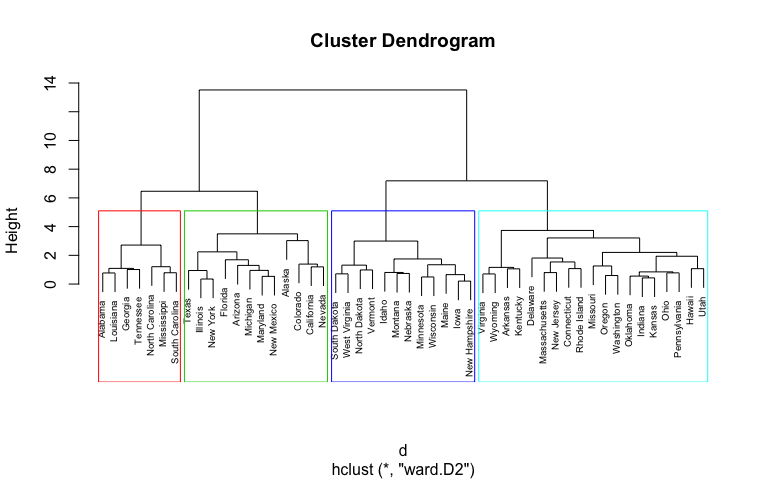
\includegraphics[width=0.8\textwidth]{images/hierarchical-clustering.png}
    \caption{Hierarchical clustering example with 4 clusters}
\end{figure}

\paragraph{Top-down clustering}
This approach starts from a cluster containing all the documents, and
recursively splits it keeping track of the parent of each document. 
The process stops when a threshold of intra-cluster similarity is obtained 
or when there's a cluster for each document.
This approach is the opposite of the bottom up tree creation.

\section{Topic modeling}

\paragraph{Vector space models problems}
The approaches seen so far did not take into 
consideration semantics of words. 
We understood that the vector space models suffer 
from high dimensionality, the terms also could be synonyms, 
leading to ambiguity, in fact two words that means 
the same thing are two different dimensions in the model.
\subsection{Linear algebra recap}

\paragraph{Eigenvalues and eigenvectors}
Given a square matrix of size $n$, if we find a
 $n$ dimensional vector such that
$$A\vec{x} = \lambda\vec{x}$$
$\lambda$ is a eigenvalue and $\vec{x}$ is an eigenvector.
It also holds that 
$$(A - \lambda I )\vec{x} = 0 \implies |A - \lambda I| = 0$$
where $I$ is the identity matrix, and the implication holds as $\vec{x}$ is non-zero.
In general the second part of the implication has $n$ solutions, so 
$n$ eigenvalues associated with a certain eigenvector.

After finding the solutions we can write that 
\begin{equation}
    \begin{aligned}
        AX &= A[\vec{x_1}, \dots, \vec{x_n}] = A\vec{x_1} + \dots + A\vec{x_n}\\
        & = \lambda_1\vec{x_1} + \dots + \lambda_n\vec{x_n} = \varLambda X  
    \end{aligned}
\end{equation}
Where $\varLambda$ is the diagonal matrix of the eigenvalues, and $X$ the matrix 
with eigenvectors. 

\paragraph{Diagonalization}
If the $n$ eigenvector found at the previous step are independent, 
and the matrix $A$ is invertible, which is not a problem as its square, 
we can write 
$$AX = X\varLambda \rightarrow AXX^{-1} = XAX^{-1} \rightarrow A = X\varLambda X^{-1}$$

This representation is called diagonalization of $A$.
Also, if $A$ is symmetric, we can write
$$A = X\varLambda X^{\top}$$

\subsection{Latent Semantic Indexing}
The goal is to discover topics that motivate data
by using matrix factorization techniques, while 
taking in consideration the possibility of expressing
the same topic with different words.

\paragraph{Idea}
We learned that if a matrix is symmetric we can write the 
diagonalization as $A = X\varLambda X^{\top}$.
The question is, what happens if we multiply the 
document-term matrix by itself? 

We find a symmetric matrix that somehow encapsulates a notion of similarity 
of documents because if two documents share the same words the 
product will be really high for that two documents.

If we multiply the term-document matrix we obtain a similar result.

\paragraph{Process}
Formally, we consider a matrix $B_{n\times n}$ as the product of the document-term 
matrix $A_{m\times n}$ by itself.
We then take the eigenvalues of the matrix $B$ and start diagonalization.

The process involves first sorting the eigenvalues, and taking the first 
$k$ non-zero ones, that will be $k$ topics we are finding in the documents, 
and we arrange the corresponding eigenvectors in $V = [\vec{v_1}, \dots, \vec{v_k}]$.

We proceed with the definition of $U = [\vec{u_1} = \frac{1}{\sigma_1}A\vec{v_1}, \dots, 
\vec{u_k} = \frac{k}{\sigma_k}A\vec{v_k}]$, that contains perpendicular $m$-dimensional 
vectors of length 1. Then we can write:
$$A = U \Sigma V^\top$$
where $\Sigma_{k \times k}$ is the diagonal matrix having $\sigma_i = \sqrt{\lambda_i}$ along the diagonal.

\paragraph{Singular value decomposition}
A more simple way of seeing the vectors introduced in the previous paragraph is:
\begin{itemize}
    \item$V$ are the eigenvectors of $AA^\top$
    \item$U$ are the eigenvectors of $A^\top A$
    \item $\Sigma$ is the diagonal matrix composed starting from the eigenvalues
    of $A A^\top$ and $A^\top A$, which are the same
\end{itemize}

\paragraph{Defining topics}
After applying singular value decomposition 
to the document term matrix we have the latent topic matrix
$\Sigma_{k \times k}$.
This matrix somehow encapsulate the top $k$ relevant topics for 
the documents, and now, to make them human understandable 
we assign each a set of words, and also, we can assign to each 
document a topic, in a soft clustering fashion.

Basically, given the three matrixes that SVD outputs, 
namely $U, \Sigma, V$, 
we can discover what topics have the documents by multiplying 
$U$ and $\Sigma$. The output will be a matrix with document 
on rows and topics on columns, where the absolute value of 
a cell represent how strong a topics is present in a document.

In the same way we can find a relation between topics and words 
by multiplying $\Sigma$ and $V^\top$.

\subsection{Latent Dirichlet Allocation}
This approach relies on probability theory to find topics
in documents. 
In the LSI approach we tried to find a \emph{glue}, formally $\Sigma$,
between document and terms.

In LDA the goal is to estimate the probabilistic relation 
between topics and documents, basically the probability that 
a given document contains a given topic, and the one that 
a topics contains a certain word.
\end{document}